% Options for packages loaded elsewhere
\PassOptionsToPackage{unicode}{hyperref}
\PassOptionsToPackage{hyphens}{url}
%
\documentclass[
]{book}
\usepackage{amsmath,amssymb}
\usepackage{lmodern}
\usepackage{iftex}
\ifPDFTeX
  \usepackage[T1]{fontenc}
  \usepackage[utf8]{inputenc}
  \usepackage{textcomp} % provide euro and other symbols
\else % if luatex or xetex
  \usepackage{unicode-math}
  \defaultfontfeatures{Scale=MatchLowercase}
  \defaultfontfeatures[\rmfamily]{Ligatures=TeX,Scale=1}
\fi
% Use upquote if available, for straight quotes in verbatim environments
\IfFileExists{upquote.sty}{\usepackage{upquote}}{}
\IfFileExists{microtype.sty}{% use microtype if available
  \usepackage[]{microtype}
  \UseMicrotypeSet[protrusion]{basicmath} % disable protrusion for tt fonts
}{}
\makeatletter
\@ifundefined{KOMAClassName}{% if non-KOMA class
  \IfFileExists{parskip.sty}{%
    \usepackage{parskip}
  }{% else
    \setlength{\parindent}{0pt}
    \setlength{\parskip}{6pt plus 2pt minus 1pt}}
}{% if KOMA class
  \KOMAoptions{parskip=half}}
\makeatother
\usepackage{xcolor}
\usepackage{color}
\usepackage{fancyvrb}
\newcommand{\VerbBar}{|}
\newcommand{\VERB}{\Verb[commandchars=\\\{\}]}
\DefineVerbatimEnvironment{Highlighting}{Verbatim}{commandchars=\\\{\}}
% Add ',fontsize=\small' for more characters per line
\usepackage{framed}
\definecolor{shadecolor}{RGB}{248,248,248}
\newenvironment{Shaded}{\begin{snugshade}}{\end{snugshade}}
\newcommand{\AlertTok}[1]{\textcolor[rgb]{0.94,0.16,0.16}{#1}}
\newcommand{\AnnotationTok}[1]{\textcolor[rgb]{0.56,0.35,0.01}{\textbf{\textit{#1}}}}
\newcommand{\AttributeTok}[1]{\textcolor[rgb]{0.77,0.63,0.00}{#1}}
\newcommand{\BaseNTok}[1]{\textcolor[rgb]{0.00,0.00,0.81}{#1}}
\newcommand{\BuiltInTok}[1]{#1}
\newcommand{\CharTok}[1]{\textcolor[rgb]{0.31,0.60,0.02}{#1}}
\newcommand{\CommentTok}[1]{\textcolor[rgb]{0.56,0.35,0.01}{\textit{#1}}}
\newcommand{\CommentVarTok}[1]{\textcolor[rgb]{0.56,0.35,0.01}{\textbf{\textit{#1}}}}
\newcommand{\ConstantTok}[1]{\textcolor[rgb]{0.00,0.00,0.00}{#1}}
\newcommand{\ControlFlowTok}[1]{\textcolor[rgb]{0.13,0.29,0.53}{\textbf{#1}}}
\newcommand{\DataTypeTok}[1]{\textcolor[rgb]{0.13,0.29,0.53}{#1}}
\newcommand{\DecValTok}[1]{\textcolor[rgb]{0.00,0.00,0.81}{#1}}
\newcommand{\DocumentationTok}[1]{\textcolor[rgb]{0.56,0.35,0.01}{\textbf{\textit{#1}}}}
\newcommand{\ErrorTok}[1]{\textcolor[rgb]{0.64,0.00,0.00}{\textbf{#1}}}
\newcommand{\ExtensionTok}[1]{#1}
\newcommand{\FloatTok}[1]{\textcolor[rgb]{0.00,0.00,0.81}{#1}}
\newcommand{\FunctionTok}[1]{\textcolor[rgb]{0.00,0.00,0.00}{#1}}
\newcommand{\ImportTok}[1]{#1}
\newcommand{\InformationTok}[1]{\textcolor[rgb]{0.56,0.35,0.01}{\textbf{\textit{#1}}}}
\newcommand{\KeywordTok}[1]{\textcolor[rgb]{0.13,0.29,0.53}{\textbf{#1}}}
\newcommand{\NormalTok}[1]{#1}
\newcommand{\OperatorTok}[1]{\textcolor[rgb]{0.81,0.36,0.00}{\textbf{#1}}}
\newcommand{\OtherTok}[1]{\textcolor[rgb]{0.56,0.35,0.01}{#1}}
\newcommand{\PreprocessorTok}[1]{\textcolor[rgb]{0.56,0.35,0.01}{\textit{#1}}}
\newcommand{\RegionMarkerTok}[1]{#1}
\newcommand{\SpecialCharTok}[1]{\textcolor[rgb]{0.00,0.00,0.00}{#1}}
\newcommand{\SpecialStringTok}[1]{\textcolor[rgb]{0.31,0.60,0.02}{#1}}
\newcommand{\StringTok}[1]{\textcolor[rgb]{0.31,0.60,0.02}{#1}}
\newcommand{\VariableTok}[1]{\textcolor[rgb]{0.00,0.00,0.00}{#1}}
\newcommand{\VerbatimStringTok}[1]{\textcolor[rgb]{0.31,0.60,0.02}{#1}}
\newcommand{\WarningTok}[1]{\textcolor[rgb]{0.56,0.35,0.01}{\textbf{\textit{#1}}}}
\usepackage{longtable,booktabs,array}
\usepackage{calc} % for calculating minipage widths
% Correct order of tables after \paragraph or \subparagraph
\usepackage{etoolbox}
\makeatletter
\patchcmd\longtable{\par}{\if@noskipsec\mbox{}\fi\par}{}{}
\makeatother
% Allow footnotes in longtable head/foot
\IfFileExists{footnotehyper.sty}{\usepackage{footnotehyper}}{\usepackage{footnote}}
\makesavenoteenv{longtable}
\usepackage{graphicx}
\makeatletter
\def\maxwidth{\ifdim\Gin@nat@width>\linewidth\linewidth\else\Gin@nat@width\fi}
\def\maxheight{\ifdim\Gin@nat@height>\textheight\textheight\else\Gin@nat@height\fi}
\makeatother
% Scale images if necessary, so that they will not overflow the page
% margins by default, and it is still possible to overwrite the defaults
% using explicit options in \includegraphics[width, height, ...]{}
\setkeys{Gin}{width=\maxwidth,height=\maxheight,keepaspectratio}
% Set default figure placement to htbp
\makeatletter
\def\fps@figure{htbp}
\makeatother
\setlength{\emergencystretch}{3em} % prevent overfull lines
\providecommand{\tightlist}{%
  \setlength{\itemsep}{0pt}\setlength{\parskip}{0pt}}
\setcounter{secnumdepth}{5}
\usepackage{booktabs}

\ifLuaTeX
  \usepackage{selnolig}  % disable illegal ligatures
\fi
\usepackage[]{natbib}
\bibliographystyle{apalike}
\IfFileExists{bookmark.sty}{\usepackage{bookmark}}{\usepackage{hyperref}}
\IfFileExists{xurl.sty}{\usepackage{xurl}}{} % add URL line breaks if available
\urlstyle{same} % disable monospaced font for URLs
\hypersetup{
  pdftitle={Deep Learning},
  hidelinks,
  pdfcreator={LaTeX via pandoc}}

\title{Deep Learning}
\author{}
\date{\vspace{-2.5em}}

\begin{document}
\maketitle

{
\setcounter{tocdepth}{1}
\tableofcontents
}
\hypertarget{bienvenida}{%
\chapter*{BIENVENIDA}\label{bienvenida}}
\addcontentsline{toc}{chapter}{BIENVENIDA}

\hypertarget{objetivo}{%
\section*{Objetivo}\label{objetivo}}
\addcontentsline{toc}{section}{Objetivo}

Brindar al participante los elementos teóricos y prácticos básicos alrededor de la programación de \emph{\textbf{REDES NEURONALES ARTIFICIALES}}. Aprenderá las definiciones y aprenderá a distinguir estrategias y diferentes soluciones a problemas que pueden resolverse con algoritmos de deep learning y aprenderá a usar el conjunto de librerías en \textbf{Python} más novedoso, estructuradas y ampliamente usadas para la creación de estructuras neuronales aplicadas a problemas predictivos, clasificación y segmentación de imagenes, series de tiempo, procesamiento de lenguaje natural (NLP), etc.

\begin{center}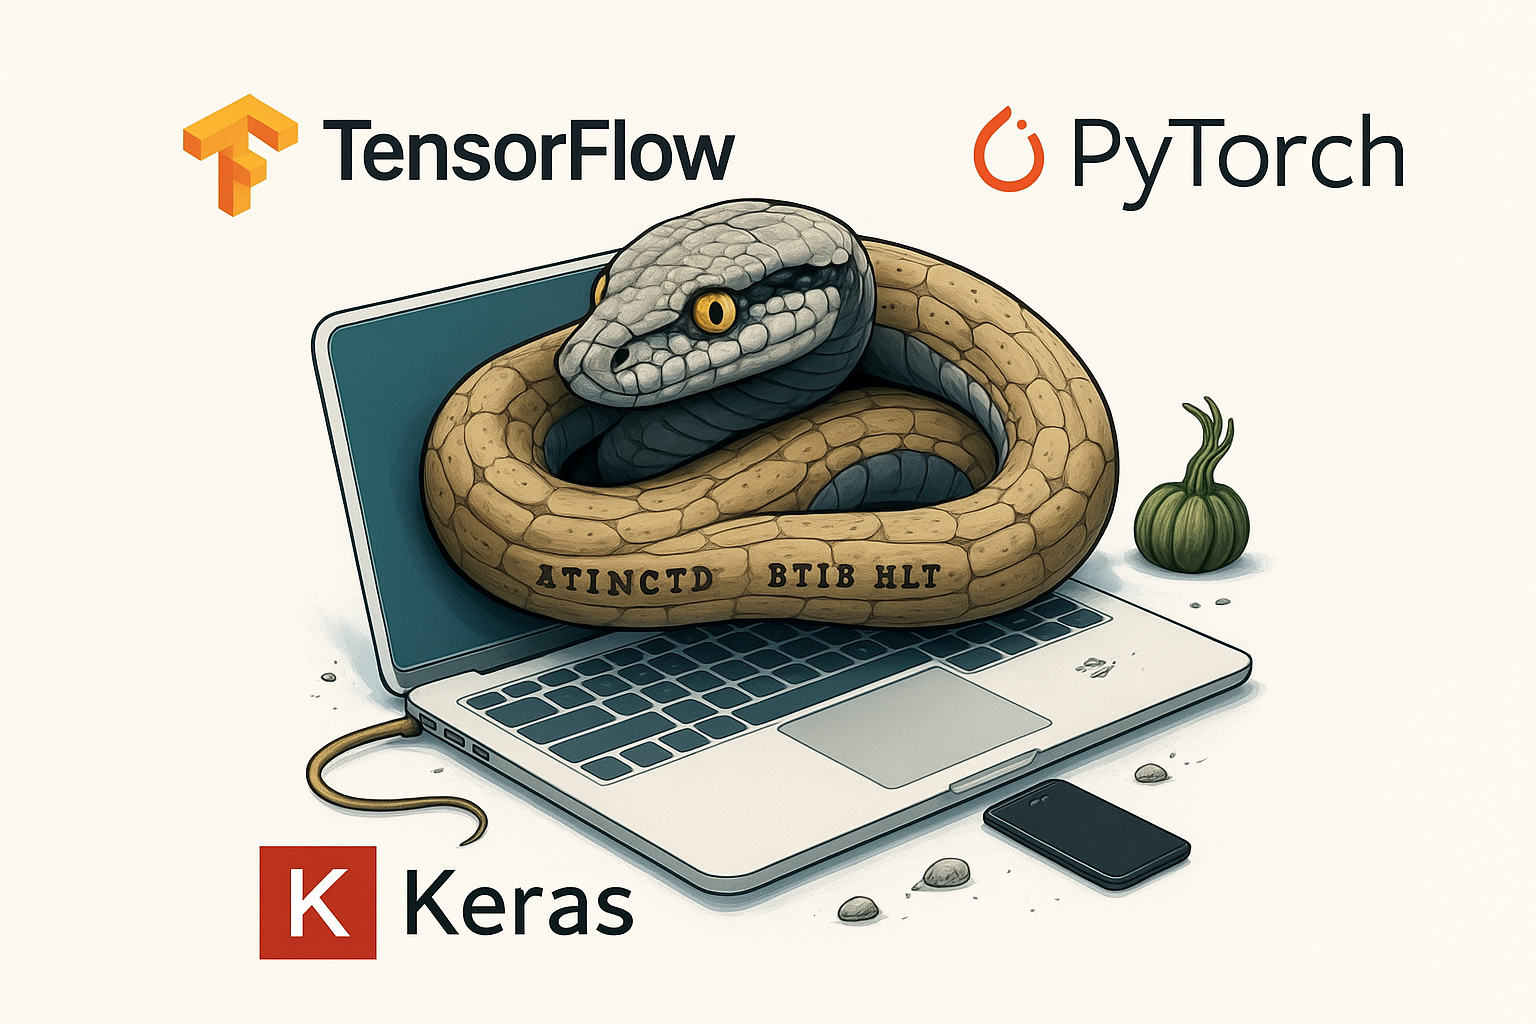
\includegraphics[width=600pt,height=350pt]{img/00-presentacion/MIT-Python-TF} \end{center}

\hypertarget{alcances-del-programa}{%
\section*{Alcances del Programa}\label{alcances-del-programa}}
\addcontentsline{toc}{section}{Alcances del Programa}

Al finalizar este curso, el participante será capaz de consumir, manipular y visualizar información para resolver problemas de propósito general asociados a los datos. Apenderá a implementar diferentes algoritmos de machine learning y mejorar su desempeño predictivo en problemas de clasificación, regresión y segmentación.

Requisitos:

\begin{itemize}
\tightlist
\item
  Computadora con al menos 8Gb Ram
\item
  Instalar Python con versión 3.11 o superior
\item
  Instalar un IDE preferido. Jupyter, RStudio, Spyder, VSCode, Colab
\end{itemize}

\hypertarget{temario}{%
\subsection*{Temario:}\label{temario}}
\addcontentsline{toc}{subsection}{Temario:}

\textbf{00. Instalación}

\textbf{01. Introducción a Deep Learning}

\textbf{02. Preliminares}

\textbf{03. Redes Neuronales Lineales para Regresión}

\textbf{04. Redes neuronales Lineales para Clasificación}

\textbf{05. Perceptrón Multicapa}

\textbf{06. Guía del Constructor}

\textbf{07. Redes Neuronales Convolucionales}

\textbf{08. Redes Neuronales Convolucionales Modernas}

\textbf{09. Redes Neuronales Recurrentes}

\textbf{10. Redes Neuronales Recurrentes Modernas}

\textbf{11. Mecanismos de Atención y Transformers}

\textbf{12. Algoritmos de Optimización}

\textbf{13. Desempeño Computacional}

\textbf{14. Visión por Computadora}

\textbf{15. Procesamiento de Lenguaje Natural: Pre-entrenamiento}

\textbf{16. Procesamiento de Lenguaje Natural: Aplicaciones}

\textbf{17. Aprendizaje por Refuerzo}

\textbf{18. Procesos Gausianos}

\textbf{19. Optimización paramétrica}

\textbf{20. Redes Generativas Adversarias}

\begin{center}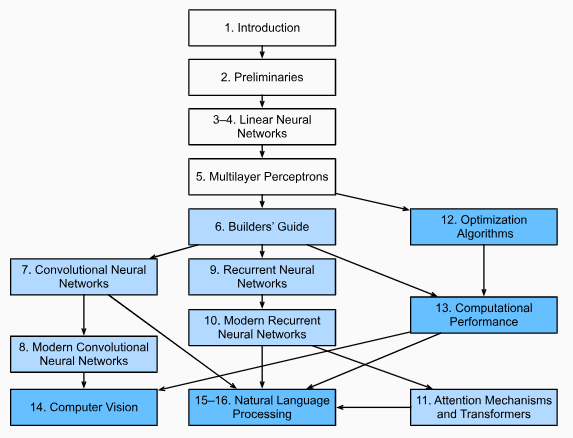
\includegraphics[width=500pt]{img/00-presentacion/estructura} \end{center}

\hypertarget{cuxf3digo}{%
\section*{Código}\label{cuxf3digo}}
\addcontentsline{toc}{section}{Código}

La mayoría de las secciones de este material presentan código ejecutable. En definitiva algunas intuiciones se desarrollan mejor mediante ensayo y error, modificando el código poco a poco y observando los resultados.

El código será presentado en chunks visibles y detacados respecto del resto del texto. Este puede ser copiador mediante el botón superior del lado derecho para su revisión y replicación en algún otro ambiente de prueba.

\begin{Shaded}
\begin{Highlighting}[]
\ImportTok{import}\NormalTok{ collections}
\ImportTok{import}\NormalTok{ hashlib}
\ImportTok{import}\NormalTok{ inspect}
\ImportTok{import}\NormalTok{ math}
\ImportTok{import}\NormalTok{ os}
\ImportTok{import}\NormalTok{ random}
\ImportTok{import}\NormalTok{ re}
\ImportTok{import}\NormalTok{ shutil}
\ImportTok{import}\NormalTok{ sys}
\ImportTok{import}\NormalTok{ tarfile}
\ImportTok{import}\NormalTok{ time}
\ImportTok{import}\NormalTok{ zipfile}
\ImportTok{from}\NormalTok{ collections }\ImportTok{import}\NormalTok{ defaultdict}
\ImportTok{import}\NormalTok{ pandas }\ImportTok{as}\NormalTok{ pd}
\ImportTok{import}\NormalTok{ requests}
\ImportTok{from}\NormalTok{ IPython }\ImportTok{import}\NormalTok{ display}
\ImportTok{from}\NormalTok{ matplotlib }\ImportTok{import}\NormalTok{ pyplot }\ImportTok{as}\NormalTok{ plt}
\ImportTok{from}\NormalTok{ matplotlib\_inline }\ImportTok{import}\NormalTok{ backend\_inline}
\end{Highlighting}
\end{Shaded}

\hypertarget{duraciuxf3n-y-evaluaciuxf3n-del-programa}{%
\section*{Duración y evaluación del programa}\label{duraciuxf3n-y-evaluaciuxf3n-del-programa}}
\addcontentsline{toc}{section}{Duración y evaluación del programa}

\begin{itemize}
\item
  El programa tiene una duración de XXX hrs.
\item
  Las sesiones serán atendidas los días XxXx, de 4:30 pm a 5:45 pm
\item
  Serán asignados ejercicios que el participante deberá resolver entre una semana y otra.
\item
  Durante todo el programa se realizarán prácticas para reforzar el aprendizaje.
\end{itemize}

\hypertarget{recursos-y-dinuxe1mica}{%
\section*{Recursos y dinámica}\label{recursos-y-dinuxe1mica}}
\addcontentsline{toc}{section}{Recursos y dinámica}

En esta clase estaremos usando:

\begin{itemize}
\tightlist
\item
  Python \href{https://www.python.org/downloads/}{da click aquí si aún no lo descargas}
\item
  RStudio \href{https://www.rstudio.com/products/rstudio/download/}{da click aquí también}
\item
  VSCode \href{https://code.visualstudio.com/download}{da click aquí si quieres descargar}
\item
  Anaconda \href{https://www.anaconda.com/download}{da click aquí si quieres descargar}
\item
  Notas de clase \href{}{Revisame si quieres aprender}
\end{itemize}

\hypertarget{part-parte-1-bases-y-preeliminares}{%
\part*{Parte 1: Bases y Preeliminares}\label{part-parte-1-bases-y-preeliminares}}
\addcontentsline{toc}{part}{Parte 1: Bases y Preeliminares}

\hypertarget{introducciuxf3n-a-deep-learning}{%
\chapter{Introducción a Deep Learning}\label{introducciuxf3n-a-deep-learning}}

\begin{Shaded}
\begin{Highlighting}[]
\ImportTok{import}\NormalTok{ numpy }\ImportTok{as}\NormalTok{ np}

\NormalTok{x }\OperatorTok{=}\NormalTok{ np.array([}\DecValTok{1}\NormalTok{,}\DecValTok{2}\NormalTok{,}\DecValTok{3}\NormalTok{,}\DecValTok{4}\NormalTok{,}\DecValTok{5}\NormalTok{])}

\BuiltInTok{print}\NormalTok{(x)}
\end{Highlighting}
\end{Shaded}

\begin{verbatim}
## [1 2 3 4 5]
\end{verbatim}

\hypertarget{preliminares}{%
\chapter{Preliminares}\label{preliminares}}

\hypertarget{redes-neuronales-lineales-para-regresiuxf3n}{%
\chapter{Redes neuronales Lineales para Regresión}\label{redes-neuronales-lineales-para-regresiuxf3n}}

\hypertarget{redes-neuronales-lineales-para-clasificaciuxf3n}{%
\chapter{Redes neuronales Lineales para Clasificación}\label{redes-neuronales-lineales-para-clasificaciuxf3n}}

\hypertarget{perceptruxf3n-multicapa}{%
\chapter{Perceptrón Multicapa}\label{perceptruxf3n-multicapa}}

\hypertarget{part-parte-2-tuxe9cnicas-modernas-de-deep-learning}{%
\part*{Parte 2: Técnicas Modernas de Deep Learning}\label{part-parte-2-tuxe9cnicas-modernas-de-deep-learning}}
\addcontentsline{toc}{part}{Parte 2: Técnicas Modernas de Deep Learning}

\hypertarget{guuxeda-del-constructor}{%
\chapter{Guía del Constructor}\label{guuxeda-del-constructor}}

\hypertarget{redes-neuronales-convolucionales}{%
\chapter{Redes Neuronales Convolucionales}\label{redes-neuronales-convolucionales}}

\hypertarget{redes-neuronales-convolucionales-modernas}{%
\chapter{Redes Neuronales Convolucionales Modernas}\label{redes-neuronales-convolucionales-modernas}}

\hypertarget{redes-neuronales-recurrentes}{%
\chapter{Redes Neuronales Recurrentes}\label{redes-neuronales-recurrentes}}

\hypertarget{redes-neuronales-recurrentes-modernas}{%
\chapter{Redes Neuronales Recurrentes Modernas}\label{redes-neuronales-recurrentes-modernas}}

\hypertarget{mecanismos-de-atenciuxf3n-y-transformers}{%
\chapter{Mecanismos de Atención y Transformers}\label{mecanismos-de-atenciuxf3n-y-transformers}}

\hypertarget{part-parte-3-escalabilidad-eficiencia-y-aplicaciones}{%
\part*{Parte 3: Escalabilidad, Eficiencia y Aplicaciones}\label{part-parte-3-escalabilidad-eficiencia-y-aplicaciones}}
\addcontentsline{toc}{part}{Parte 3: Escalabilidad, Eficiencia y Aplicaciones}

\hypertarget{algoritmos-de-optimizaciuxf3n}{%
\chapter{Algoritmos de Optimización}\label{algoritmos-de-optimizaciuxf3n}}

  \bibliography{book.bib,packages.bib}

\end{document}
